% =====================================================================
%  Phase-2 Attention-Pruning analysis — slide deck
%  Compile:  tectonic prune_analysis.tex   (auto-fetches metropolis)
%  Data: attention_prune/analyze_prune_k1.py  (single-seed k=1, n=1663)
% =====================================================================
\documentclass[aspectratio=169]{beamer}
\usetheme{metropolis}
\usepackage{booktabs}\usepackage{xcolor}\usepackage{array}\usepackage{colortbl}
\usepackage{graphicx}\usepackage{pifont}
\definecolor{good}{HTML}{2E7D32}\definecolor{bad}{HTML}{C62828}\definecolor{accent}{HTML}{1565C0}
\definecolor{ours}{HTML}{0D47A1}\definecolor{warn}{HTML}{FFB300}
\setbeamercolor{frametitle}{bg=accent}
\setbeamerfont{frametitle}{size=\large}
\newcommand{\yes}{\textcolor{good}{\textbf{supported}}}
\newcommand{\parttok}{\textcolor{warn}{\textbf{partial}}}
\newcommand{\no}{\textcolor{bad}{\textbf{not supported}}}
\newcommand{\ci}[2]{{\scriptsize[#1,\,#2]}}

\title{Is the 360\textdegree{} street view redundant?}
\subtitle{Phase-2 attention pruning --- Qwen3.6-27B, $k{=}1$, $n{=}1663$ solved questions}
\date{}\author{}
\begin{document}
\maketitle

% ---------------------------------------------------------------------
\begin{frame}{The claim under test}
\large
Each urban VQA question shows \textbf{4 street-view cameras}
(\texttt{fwd}, \texttt{bwd}, \texttt{cross\_left}, \texttt{cross\_right}).
\vspace{4pt}
\begin{block}{Claim}
For 8 urban-attribute MCQ tasks, the full 360\textdegree{} view is \textbf{redundant}:
the \textbf{1 image the model attends to most} keeps the answer correct ---
and that image is the \textbf{forward camera}.
\end{block}
\vspace{4pt}
\footnotesize
\textbf{Setup.} Solve on 4 images $\to$ keep only $k{=}1$ image per arm $\to$ re-ask greedily.
\textbf{Survival \%} = of questions solved on 4 images, fraction still correct on the kept image
(a per-question \emph{ceiling}, never a raw accuracy).
\par\vspace{2pt}
\textbf{Arms:} \textcolor{ours}{top} (most-attended) $\,\vert\,$ \textcolor{accent}{fwd} (always forward)
$\,\vert\,$ random $\,\vert\,$ \textcolor{bad}{bottom} (least-attended) $\,\vert\,$ zero (no image = leakage probe).
\end{frame}

% ---------------------------------------------------------------------
\begin{frame}{Verdict in one slide}
\centering\small
\begin{tabular}{p{6.4cm} c p{4.2cm}}
\toprule
Claim & Verdict & Key number \\
\midrule
\textbf{A.} 360\textdegree{} redundant; \emph{one} image often enough & \yes &
 top $89.5\%$ \ci{88.0}{90.9}; even random $82.1\%$ \\[3pt]
\textbf{B.} Attention \emph{ranking} selects the right image & \parttok &
 top$-$random $+7.4$ \ci{+5.0}{+9.8}, \textbf{but} top$\approx$fwd \\[3pt]
\textbf{C.} The image that matters is the \emph{forward} camera & \yes &
 fwd $89.1\%$ \ci{87.5}{90.5}; attn.\ \#1 $=$ fwd $94.8\%$ \\
\bottomrule
\end{tabular}
\vspace{8pt}
\begin{block}{One line}
\small The 360\textdegree{} view \textbf{is} redundant and a \textbf{single forward image} usually suffices.
Attention beats random selection --- but only because it \textbf{almost always points at the forward camera}.
No evidence (at this power) that the \emph{ranking} adds anything beyond ``use forward.''
\end{block}
\end{frame}

% ---------------------------------------------------------------------
\begin{frame}{Pooled survival --- one image is usually enough}
\centering
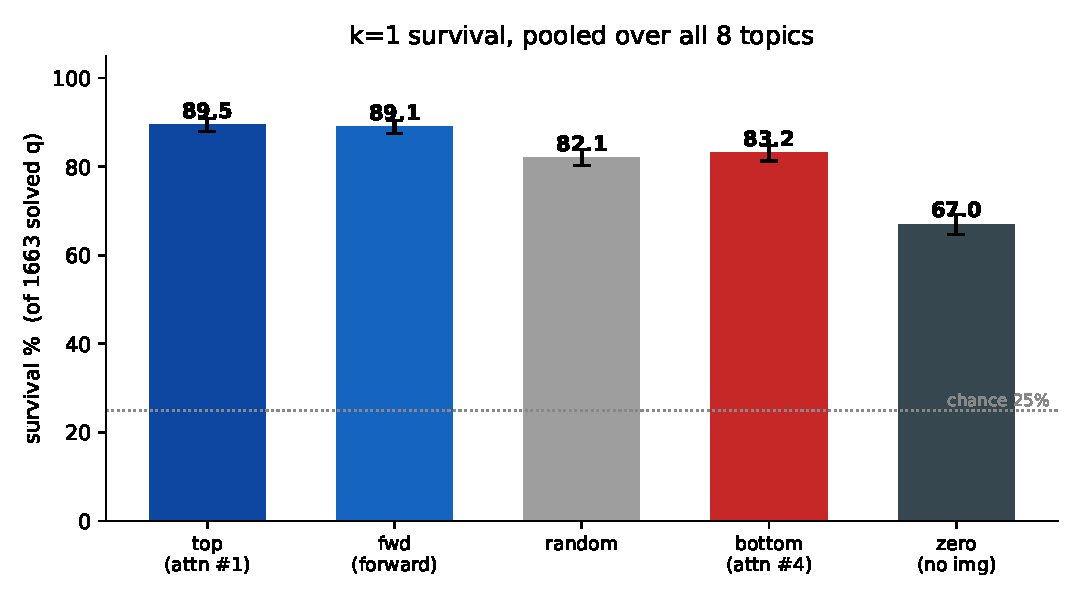
\includegraphics[width=0.74\linewidth]{figures/prune_pooled.pdf}
\par\vspace{2pt}
\footnotesize
\textcolor{ours}{top}$=$\textcolor{accent}{fwd}$\gg$random$\approx$\textcolor{bad}{bottom}$\gg$zero.
Even the \emph{least}-attended image survives $83.2\%$ --- ``even the worst single view is usually enough.''
\end{frame}

% ---------------------------------------------------------------------
\begin{frame}{The leakage problem dominates everything}
\small
6 of 8 topics are answerable from \textbf{text + options alone}. The \textbf{zero} arm
(no image) is the empirical detector:
\vspace{2pt}
\begin{center}\scriptsize
\begin{tabular}{lcc|lcc}
\toprule
topic & blind & zero-surv & topic & blind & zero-surv \\
\midrule
road\_surface & 0.957 & \textbf{96.4\%} & land\_use & 0.523 & 73.8\% \\
junction\_type & 0.614 & 49.1\% & \textcolor{good}{amenity\_richness} & \textcolor{good}{0.373} & 51.3\% \\
road\_type & 0.603 & 59.4\% & \textcolor{good}{transit\_density} & \textcolor{good}{0.297} & \textbf{84.6\%}(!) \\
urban\_density & 0.546 & 62.3\% & building\_height & 0.474 & 51.5\% \\
\bottomrule
\end{tabular}
\end{center}
\vspace{2pt}
\begin{itemize}\footnotesize
\item Pooled \textbf{zero}-image survival is \textbf{67\%} --- most ``survival'' is \emph{not} image use.
\item Only \textcolor{good}{\textbf{amenity\_richness}} and \textcolor{good}{\textbf{transit\_density}}
 (blind $<0.45$) carry the headline. The other six are reported but \textbf{excluded}.
\item Even a ``safe'' topic (transit) survives $84.6\%$ with \textbf{zero} images.
\end{itemize}
\end{frame}

% ---------------------------------------------------------------------
\begin{frame}{Per-topic --- top vs zero vs blind prior}
\centering
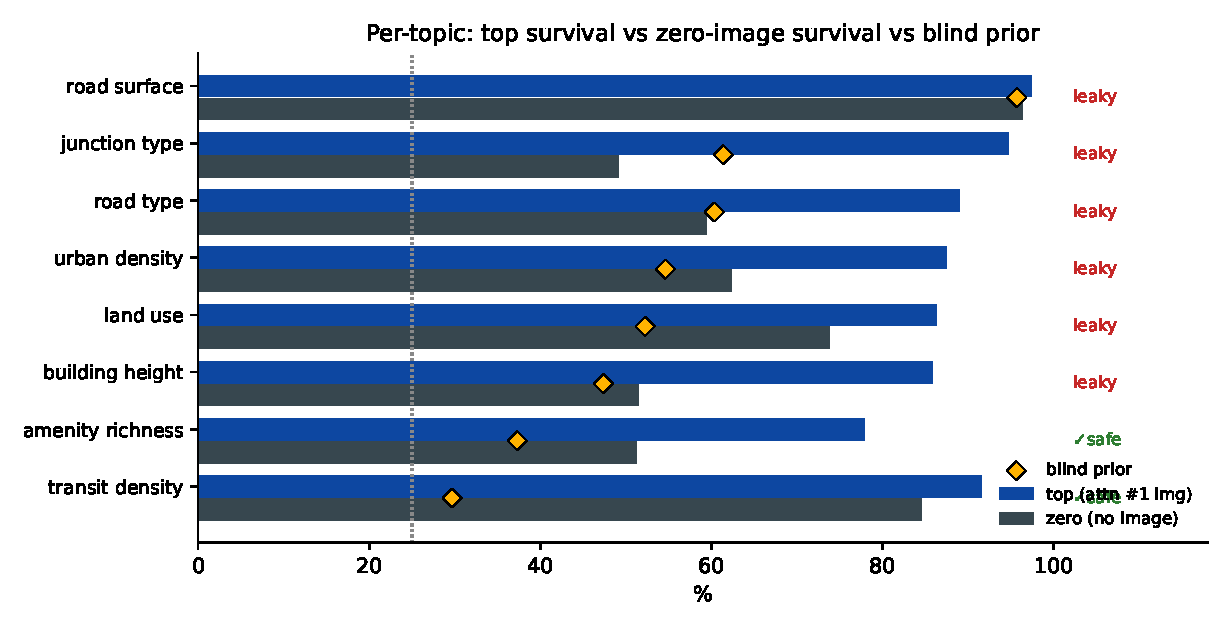
\includegraphics[width=0.80\linewidth]{figures/prune_pertopic.pdf}
\par
{\footnotesize Sorted by blind prior. \texttt{road\_surface}: top survival rides almost entirely on the
$0.957$ prior (zero already $96.4\%$) --- \textbf{no} image signal.}
\end{frame}

% ---------------------------------------------------------------------
\begin{frame}{Honest headline: condition on questions that NEED an image}
\footnotesize
Cleanest test --- restrict to the \textbf{zero-FAIL} subset (model wrong with no image), leakage-safe pool:
\begin{center}
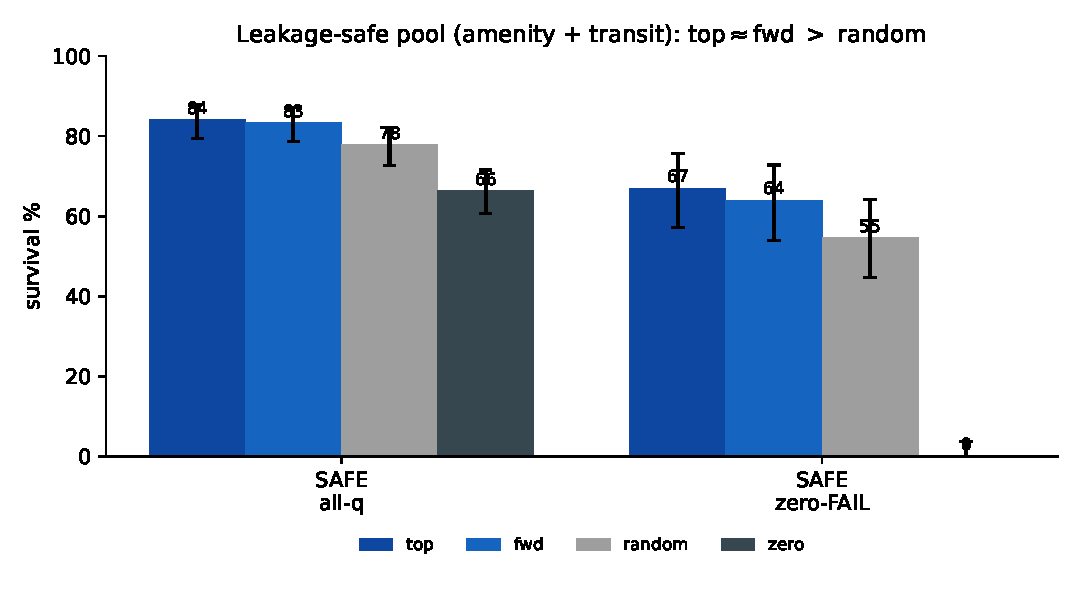
\includegraphics[width=0.55\linewidth]{figures/prune_safe.pdf}
\end{center}
\vspace{-4pt}
\begin{itemize}
\item top$\approx$fwd clearly above random/zero --- redundancy $+$ ``forward matters'' \textbf{hold} on the clean pool.
\item \textbf{But} gap(top$-$random) $=+6.2$ \ci{-0.2}{+12.6} (all-q), $+12.4$ \ci{-1.3}{+25.4} (zero-FAIL):
 \textcolor{bad}{\textbf{CI includes 0 --- not significant}} ($n{=}288/97$).
\end{itemize}
\end{frame}

% ---------------------------------------------------------------------
\begin{frame}{Does the attended image beat a random one?}
\centering
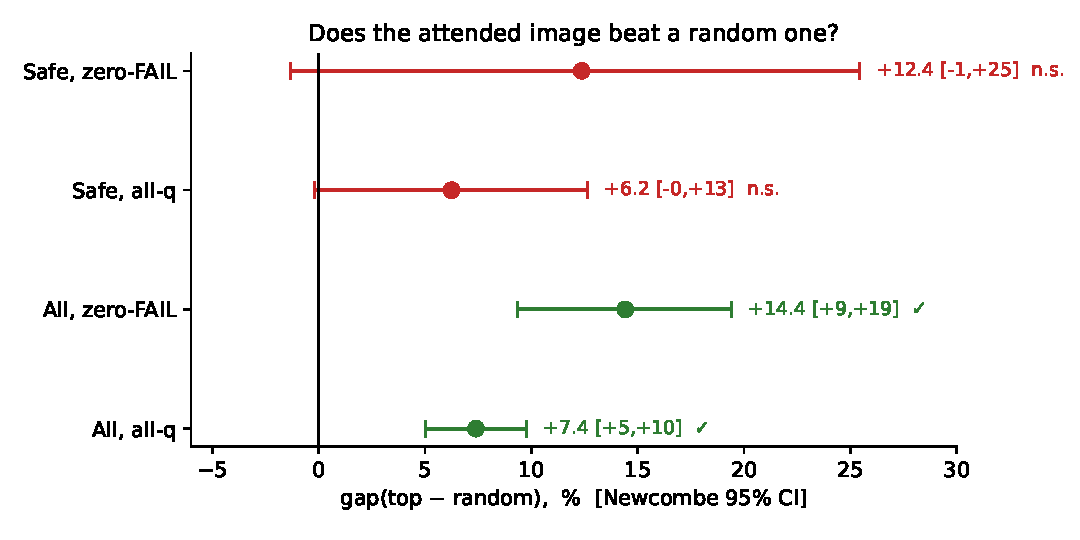
\includegraphics[width=0.78\linewidth]{figures/prune_gap.pdf}
\par\vspace{2pt}
\footnotesize
Gap is \textbf{real \& significant on the full pool} (and \emph{grows} on zero-FAIL: leakage doesn't
explain it). On the clean 2-topic safe pool it is \textbf{only suggestive} --- small $n$.
\end{frame}

% ---------------------------------------------------------------------
\begin{frame}{top vs fwd: does attention earn its keep?}
\small
Attention's \#1 image \textbf{is the forward camera in $94.8\%$} of questions.
It disagrees in only \textbf{86 / 1663}.
\vspace{4pt}
\begin{center}\small
\begin{tabular}{lccc}
\toprule
scope & top & fwd & gap(top$-$fwd) \\
\midrule
all pool ($n{=}1663$) & $89.5\%$ & $89.1\%$ & $+0.5$ \ci{-1.6}{+2.6} \;\textcolor{bad}{n.s.} \\
attn.\ $\neq$ fwd ($n{=}86$) & $82.6\%$ & $73.3\%$ & $+9.3$ \ci{-3.2}{+21.4} \;\textcolor{bad}{n.s.} \\
\bottomrule
\end{tabular}
\end{center}
\vspace{4pt}
\begin{block}{Honest reading}
\small The ``attention selects the right image'' claim \textbf{collapses into} ``keep the forward image.''
When attention \emph{disagrees} with forward it \emph{may} win ($+9.3$ pts) --- but $n{=}86$ is too small to prove it.
\textbf{That 86-question subset is where a larger run earns the stronger claim.}
\end{block}
\end{frame}

% ---------------------------------------------------------------------
\begin{frame}{Adversarial checks (tried to break it)}
\small
\begin{itemize}
\item \textbf{Leakage cancellation?} No --- gap \emph{grows} on image-dependent subset
 ($+7.4\to+14.4$). Real signal.
\item \textbf{bottom $\geq$ random?} Tie: $+1.0$ \ci{-1.6}{+3.6}. Verified \textbf{not} a bug ---
 bottom kept the rank-4 image in \textbf{1663/1663}. Supports redundancy.
\item \textbf{Position confound.} \texttt{fwd} kept partly for its fixed grid slot;
 cannot separate content from position. \textbf{Stated, not resolved} (fwd success
 ranges $51\!-\!98\%$ across topics $\Rightarrow$ tracks content somewhat).
\item \textbf{CI discipline.} Wilson/Newcombe on every rate \& gap; CI-includes-0 marked n.s.
\item \textbf{$k$-monotonicity.} \textbf{Untestable} --- only $k{=}1$ complete.
\end{itemize}
\end{frame}

% ---------------------------------------------------------------------
\begin{frame}{Limitations (be skeptical)}
\small
\begin{enumerate}
\item \textbf{Leakage dominates} --- 6/8 topics text-solvable; pooled zero-survival $67\%$.
 Headline rests on 2 topics, where the gap is \emph{not} significant.
\item \textbf{$k{=}1$ only} --- no $k{=}2/3$ curve; the ``1--3 images'' claim is half-tested.
 (Multi-seed/$k$ run is $2.1\%$ done $\to$ unusable.)
\item \textbf{Single random seed (3407)} --- no per-seed spread.
\item \textbf{Position confound} on the forward camera.
\item \textbf{Solver $=$ 27B $\neq$ deployed model} --- survival is a ceiling for this solver.
\item \textbf{Selection bias} --- pool $=$ questions solved on 4 images (conditional).
\item \textbf{Single-token attention} --- \texttt{choice}$\equiv$\texttt{avg}; ranking is one
 across-layer mean, a coarse signal.
\end{enumerate}
\end{frame}

% ---------------------------------------------------------------------
\begin{frame}{Take-home}
\Large
\begin{itemize}
\item[\textcolor{good}{\ding{51}}] 360\textdegree{} is \textbf{redundant}; \textbf{one} street-view image usually suffices.
\item[\textcolor{good}{\ding{51}}] That image is the \textbf{forward camera} (\texttt{along\_fwd}).
\item[\textcolor{warn}{$\sim$}] Attention \textbf{beats random}, but mostly \emph{because} it picks forward ---
 ``attention selects the right image'' is \textbf{not} yet earned.
\end{itemize}
\vspace{6pt}
\normalsize
\centering\footnotesize
Repro: \texttt{python attention\_prune/analyze\_prune\_k1.py} \;|\; analysis sha \texttt{b083f41}
\;|\; $n{=}1663$, seed 3407.
\end{frame}

\end{document}
